\section{Methods}
Studying the dynamics of solid-state systems far from equilibrium with ultrafast experimental techniques has gained attraction over the last decades.
These techniques allow probing different observables on femtosecond timescales, shedding light on the relaxation pathways towards equilibrium.

\subsection{Pump-probe Experiments}
A simple concept to reach high time resolutions is the pump-probe technique.
The basic idea is that an excitation (pump) event and a probe event with a known variable time difference occur on the sample under investigation.
The excitation event may be an arriving optical laser pulse and the probe event might be the scattering of an electron or X-ray pulse.
If probe-events are measured while continuously varying the time delay, the data can be assembled into a \emph{movie}.
Both, excitation and probe event, are required to be shorter than the timescale of the phenomenon under investigation.
If the phenomenon under study is reversible and there is enough time between each excitation event, a measurement can be done continuously on one sample.
Current plans do not involve studying irreversible phenomena.

\begin{figure}[!t]
	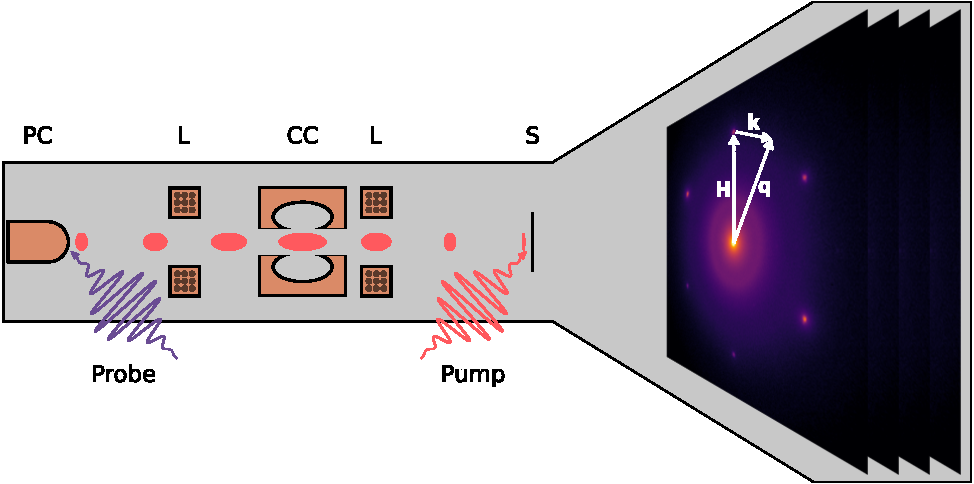
\includegraphics[width=\columnwidth]{figs/ued.pdf}
	\caption{Schematic of the UED/UEDS experiment with Photocathode~(PC), two electromagnetic Lenses~(L), compression cavity~(CC) and sample~(S). The 266\,nm ultraviolet laser pulse hits the photocathode emitting electrons that are accelerated by a static electric field towards the sample. Two lenses and the cavity focus and compress the electron bunches onto the sample where they are diffracted. The 800\,nm pump pulse arrives at the sample with variable time delay and photoexcites it. The vectors on the diffraction image are the scattering vector~$\mathbf{q}$, the reduced wave vector~$\mathbf{k}$ and the position of the closest Bragg spot $\mathbf{H}$.}
	\label{fig:ued}
\end{figure}

\subsection{Ultrafast Electron Diffraction and Ultrafast Electron Diffuse Scattering}
Building on the idea of the pump-probe scheme one can combine classical electron diffraction experiments and femtosecond laser systems to conduct \ac{UED} and \ac{UEDS} experiments.

\subsubsection*{Experimental Setup}
The experimental apparatus starts with a commercial Ti:sapphire laser system emitting $\sim$35\,fs laser pulses at a repetition rate of 1\,kHz with a center wavelength of 800\,nm, that are split and guided onto different beam path\cite{chatelain2012}.
For sample excitation, one part of the pulses is attenuated and guided onto the sample.
The second part of the pulses are entering the probe beam path and are frequency doubled. The fundamental and frequency doubled pulses are converted to a pulse with a center wavelength of 266\,nm by frequency summation.
The final pulse is guided into the vacuum part of the apparatus that is depicted in figure~\ref{fig:ued}.
It first hits the photo cathode, where the electron bunch that will later be scattered from the sample is being created.
The electron bunch is accelerated to 90\,keV by a static electric field and focused onto the sample.
On its way to the sample the electron bunch broadens considerably due to Coulomb repulsion, effectively limiting the time resolution of the experiments.
The dispersion of the electron bunch is inherently linear; fast electrons are in front, while slow electrons are in the back.
To compensate for the broadening the electron bunches are compressed in a radio-frequency driven cavity between the electron gun and the sample\cite{otto2017}.
While passing the cavity the electric field decelerates the electrons in the front and accelerates the electrons in the back.
Center electrons experience no energy change, since the radio-frequency field changes sign and is zero at that exact moment.
The electron bunch leaving the cavity now has a reverse linear dispersion and re-compresses while it is traveling through the instrument.
Maximum compression occurs right at the sample resulting in maximum time resolution.
Photoexcitation happens upon arrival of the 800\,nm pump pulse before probing sample with the compressed electron bunch.
The scattering patterns are collected in a transmission geometry; Continuously varying the time delay allows to assemble a \emph{diffraction movie} and investigate dynamics of the probed system.

Electron diffraction experiments done in transmission naturally require the samples to be transparent for electrons.
Methods of preparing thin samples of layered materials like \acp{TMD} include exfoliation\cite{mak2010} and ultramicrotomy\cite{malis1990}.
Both methods are established and available in the Sample Preparation Lab of McGill's Physics Department.
Due to the layered structure the samples' surfaces will be parallel to the monolayers.
When conducting experiments with the electron bunches arriving normal to \ts\space samples and it's layers, the $\Gamma\mathrm{MK}$ plane of the \ac{BZ} is probed.
In order to probe the L points of \ts\space the sample needs to be tilted by 27\textdegree.
However, tilting the sample will decrease the time-resolution of the instrument, because electron and light pulse travel at different speeds.
Estimating the electron spot size on the sample to be 400\,µm, the electron velocity of electrons with an energy of 90\,keV to be half the speed of light, the deviation in probed time delays across the sample area tilted by 27\textdegree will be about 340\,fs.
Time-resolved experiments will still be very much feasible, albeit with a limited time resolution; an approach to account for this problem will be presented in the outlook of this document.

\subsubsection*{Information Encoded in Scattering Data}
The datasets collected are incredibly rich and contain information about wave-vector-dependent dynamics of the phonon system across the whole \ac{BZ}.
The total scattering intensity collected on the detector is in the kinematic approximation
\begin{equation} I(\mathbf{q},t) = \sum_n I_n(\mathbf{q},t)\enspace\text{with}\enspace n \in\mathbb{N}^0\,\label{eq:I}\text{\cite{renedecotret2019}},\end{equation}
with the scattered intensities $I_n$ of an electron that scattered with $n$ phonons at scattering vector $\mathbf{q}$ at time~$t$.
Contribution to the scattered intensity decreases rapidly for higher order terms, hence only the first two terms will be discussed in detail.

The first term describes the intensity of the electrons diffracted into Bragg spots with the proportionality
\begin{equation} I_0(\mathbf{q}, t) \propto \left| \sum_s f_s(\mathbf{q}) \e^{-W_s(\mathbf{q},t)} \e^{-\i[\mathbf{q}\cdot\mathbf{R}_s(t)]} \right| ^2.\label{eq:I0}\end{equation}
The sum expression is the so-called geometric structure factor and contains the atomic form factors $\{f_s(\mathbf{q})\}$ determined by the scattering potential of each atomic species.
Other terms are the Debye-Waller factors $\{\e^{-W_s(\mathbf{q},t)}\}$ and phase factors $\{\e^{-\i[\mathbf{q}\cdot\mathbf{R}_s(t)]}\}$ with the atomic positions in the unit cell $\{\mathbf{R}_s(t)\}$, $s$ is running over the atoms in the unit cell.
Direct calculation of the real space structure of the sample from the experimental data is impossible, since the phase factor information is lost due to the absolute square.
Information about thermal motion of the atoms is encoded in the Debye-Waller factor.
It is proportional to the mean square atomic displacement of the atoms around their equilibrium position, thus containing information on all phonon modes, but it is not possible to disentangle them.
The factor leads to an intensity reduction of the Bragg spots.

To track the phonon dynamics in more detail, namely in energy, momentum and time, one must also consider the intensity of scattering events involving one phonon

\begin{equation} I_1(\mathbf{q},t) \propto \sum_i \frac{n_{i,\mathbf{k}}(t)+\frac{1}{2}}{\omega_{i,\mathbf{k}}(t)}\,\left| F_{1,i}(\mathbf{q},t) \right|^2 = \sum_i \frac{n_{i,\mathbf{k}}(t)+\frac{1}{2}}{\omega_{i,\mathbf{k}}(t)}\,\left| \sum_s \e^{-W_s(\mathbf{q},t)} \frac{f_s(\mathbf{q})}{\sqrt{\mu_s}} \left( \mathbf{q}\cdot\mathbf{e}_{i, s}(\mathbf{k}) \right) \right|^2.\label{eq:I1}\end{equation}
The index of the outer sum $i$ runs over all phonon modes populations $\{n_{i,\mathbf{k}}\}$ and their respective frequencies $\{\omega_{i,\mathbf{k}}\}$.
$\left| F_{1,i}(\mathbf{q},t) \right|^2$ is the one-phonon structure factor and weighs the contribution of each phonon mode~$i$ to the first order diffuse scattering intensity.
In full, the one-phonon structure factor is written on the RHS of equation~\ref{eq:I1} with index~$s$ running over the atoms in the unit cell and the Debye-Waller and the atomic form factors from equation~\ref{eq:I0} and the atomic masses $\{\mu_s\}$ and the phononic polarization vectors $\{\mathbf{e}_{i, s}(\mathbf{k})\}$.
To track the flow of energy in the sample after optical excitation access to the changes in population dynamics across the \ac{BZ} is important.
In order to derive $\{n_{i,\mathbf{k}}(t)\}$ from the first-order diffuse scattering intensity, one must obtain knowledge of the one-phonon scattering factors and the phonon frequencies.
A extensive description on how to calculate the $\left| F_{1,i}(\mathbf{q},t) \right|^2$ and finally electron-phonon coupling constants is presented in~\cite{stern2018,renedecotret2019}.

\begin{figure}[!t]
	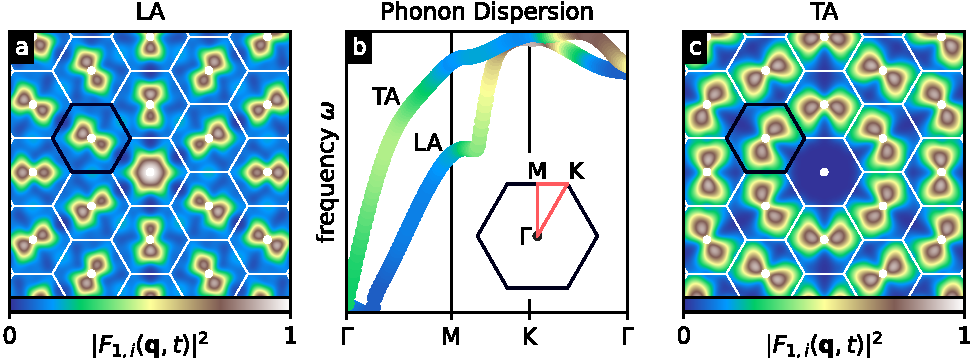
\includegraphics[width=\columnwidth]{figs/ops.pdf}
	\caption{One-phonon structure factor of the longitudinal~(\textbf{a}) and transverse~(\textbf{c}) acoustic phonon modes in the high temperature phase of \ts over reciprocal space. Withe dots mark $\Gamma$ points and white lines mark \ac{BZ} edges. \textbf{b})~Phonon dispersion of the along the high-symmetry path $\overline{\Gamma\mathrm{MK}\Gamma}$. The graphs colors are visualizing the value of the corresponding one-phonon structure factor for every point in reciprocal space, taken from the \ac{BZ} marked by black edges in \textbf{a} and \textbf{c}. The single \ac{BZ} inset is showing the cut through the \ac{BZ} with a red line.}
	\label{fig:ops}
\end{figure}

In summary: \Ac{DFT} calculations and clustering algorithms are used to obtain the polarization $\mathbf{e}_{i,s,\mathbf{k}}$ and frequency $\omega_{i,\mathbf{k}}$ of phonon states across the \ac{BZ} and sort them into branches.
Any transient changes in the Debye-Waller factor are negligible and can be therefore obtained from the static phonon polarizations calculated by the \ac{DFT} calculation.
The calculations were carried out for the high temperature phase of \ts at room temperature and parts of the result are shown in figure~\ref{fig:ops}.
Panel~a~and~c show the one-phonon structure factor across multiple \acp{BZ} for the \ac{LA} and \ac{TA} mode respectively.
Frequencies of both modes across the high-symmetry path $\overline{\Gamma\mathrm{MK}\Gamma}$ are reported in panel~b.
Encoded in the color of the lines is the value of the one-phonon structure factor in the \acp{BZ} with the black borders.
Lets discuss the implications of the scalar product $\left( \mathbf{q}\cdot\mathbf{e}_{i, s}(\mathbf{k}) \right)$ in equation~\ref{eq:I1} for the structure factors of longitudinal and transverse phonon modes qualitatively.
For transverse phonon modes the structure factor is large from the $\Gamma$ point along the azimuthal direction, because the mode polarization is perpendicular to $\mathbf{q}$.
Vice versa the polarization of the longitudinal modes is parallel to $\mathbf{q}$ and the structure factor exhibits prominent features radially.
With the frequencies and one-phonon structure factor on hand the derivation of the phonon populations $\{n_{i,\mathbf{k}}(t)\}$ is straightforward.
Employing the so-called nonthermal lattice model\cite{waldecker2016} (a set of coupled equations, with a temperature and a heat capacity assigned to the electron system and each phonon mode) allows the determination of electron-phonon coupling constants.

In 2021 Zacharias et~al. published methods to extend the presented calculation to multi-phonon structure factors of orders $n\geq 2$ (see equation~\ref{eq:I}).
Further they compare the theoretical results with experimental data on different 2D-materials, including \acp{TMD}, showing good agreement\cite{zacharias2021a,zacharias2021b}.

%capabilities of the machine
% photoexcitation absorbed by electrons
%peak width <-> correlation length